\documentclass{article}
\usepackage{amsmath,graphicx,mlspconf}
\usepackage[english]{babel}
\usepackage[colorlinks=true, allcolors=blue]{hyperref}



% Title.
% ------
\title{A Machine Translation Model for French to English with BLEU Score}
\name{Dhruv Jain, Sunday Okechukwu }


\begin{document}

\maketitle

\begin{abstract}

Machine translation is an essential technology for breaking language barriers and fostering cross-cultural communication.
Loosely speaking Machine Translation refers to the automated process of translating text or speech from one language called (source language) to another language called (target language). For eg. frn-eng or spn-eng.
Technically, it involves training machine learning models on large datasets of parallel text, where the same text is available in two or more languages
In this paper, we present a machine translation model that translates French sentences into English using an encoder - decoder architecture with BLEU metric for evaluations. The encoder and decoder is built by stacking LSTMs. We use this type of layer because its structure allows the model to understand context and temporal dependencies of the sequences.

The model is trained on a large dataset of pre-processed French and English sentence pairs. The LSTM neural network model is used to learn the underlying patterns in the dataset and generate English translations for new French sentences. The model is trained to optimize the BLEU score, a widely-used metric for evaluating the quality of machine translation systems.


\end{abstract}
%
\begin{keywords}
BLEU, LSTM, French language, Englisgh language  
\end{keywords}

\section{Introduction}

Language is a system of communication used by a particular country or community. considering language as a barriers from one country to another country. English is the most popular language world wide and its user are billions. French is the fifth most popular language across the world and its users are around 275+ millions. Looking into this we are finding a solution that can help a lot of foreign treaty to solve this problem using the model provided by Dhruv and Sunday.

The basic idea is to convert the french words to English using Natural language process and implementing the different strategies to get the best performance evaluation for this project. French to English translation using BLEU model evaluation is an automated translation system that uses a Long Short-Term Memory (LSTM) neural network model to translate French sentences into English. The system calculates the Bilingual Evaluation Understudy (BLEU) score, a widely-used metric for evaluating the quality of machine translation, to measure the accuracy of the translations. The model is trained to predict the English translation of a given French sentence by learning the underlying patterns in the data set. Once trained, the model can be used to translate new French sentences into English. This system has potential applications in various domains, including language learning, cross-cultural communication, and international business.

\textbf{Main stages of the Project} \\
- Data Acquisition \\ 
- Pre-processing \\ 
- Feature Extraction \\
- Modelling \\
- Evaluations \\
- Summary and direction for future work \\

\subsection{All about data set }

The data Acquisition collected from \\
\url{https://www.statmt.org/europarl/}. \\
This is a huge data set contains 15215 unique words in english and 29251 unique words in french. The data after loading looks like this: 

\begin{figure}[htp]
    \centering
    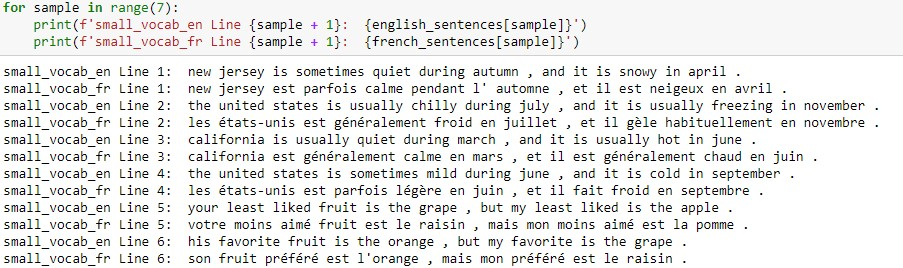
\includegraphics[width=8.5cm]{1.jpg}
    \caption{French and English sentence by sentence}
    \label{fig:galaxy}
\end{figure}


\subsection{Data Acquisition}

We started with a small dataset and use some tricks to create more data. Randomly select words in a sentence and trying the model accuracy. Take a uni gram, bi gram, tri gram, four gram for evelauting model.Back translation was used but the model is giving us a decent accuracy using BLEU model. \cite{zou2013bilingual}

\begin{figure}[htp]
    \centering
    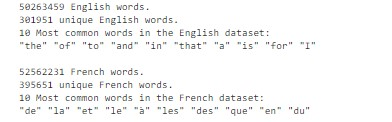
\includegraphics[width=8.5cm]{2.jpg}
    \caption{French and English Word Frequencies: Most Common Words}
    \label{fig:galaxy}
\end{figure}


\subsection{Text cleaning}
The data collected does not required any data cleaning. The data doesn't contain any NA/missing values plus the french translation has more words in the model.  

\subsection{Pre-processing}
We followed some some basic text pre processing:
Lowering the text, puncuation, Padding. From sentences to word and assigning the words to a number for each sentence. From the below a mtrix is further created and the max number of lenght in sentences was 200 words. 

\begin{figure}[htp]
    \centering
    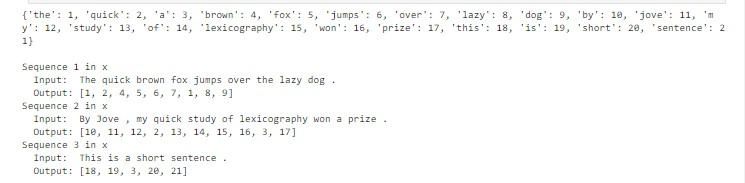
\includegraphics[width=8.5cm]{3.jpg}
    \caption{Assigning each words a unique number}
    \label{fig:galaxy}
\end{figure}


Since a majority of the pipeline is built with language specific tools, what will happen to our NLP pipeline, which is expecting English text? In such cases, language detection is performed as the first step in an NLP pipeline.Many people across the world speak more than one language in their day-to-day lives. Thus, it's not uncommon to see them using multiple languages in their social media posts, and a single post may contain many languages.

\textbf{Input sequence} length in machine translation, the length of the input sequence can vary from one sentence to another. However, neural networks are designed to work with fixed-length inputs. Padding is used to make all input sequences of the same length, which allows them to be processed in batches, making training more efficient.

\textbf{Output sequence }length similar to the input sequence length, the length of the output sequence can also vary. In order to generate an output sequence of the desired length, padding is used to ensure that all output sequences are of the same length.\\
Overall, padding is necessary in machine translation to ensure consistency in input representation, facilitate efficient computation, and enable the use of batch processing during training.


\begin{figure}[htp]
    \centering
    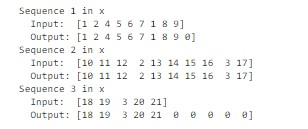
\includegraphics[width=8.5cm]{4.jpg}
    \caption{Padding}
    \label{fig:galaxy}
\end{figure}

\subsection{Feature engineering}

Tokenization is the process of splitting a sentence or a piece of text into individual words, which are called tokens. In the context of language translation from French to English, word-level tokenization is an important pre-processing step that is used to convert the input text into a format that can be processed by a machine learning model. In tokenization, each word in the input text is treated as a separate token.Each of these words is considered a separate token, which can then be used as input to a machine learning model for language translation.

Here, instead of using pre-trained word embeddings such as GloVe. We shall train our own embeddings using Keras embedding layer. Word embeddings can be thought of as an alternate to one-hot encoding along with dimensionality reduction.

Embedding layer enables us to convert each word into a fixed length vector of defined size.

There are three parameters to the embedding layer. \\
\textbullet  Input dim : Size of the French vocabulary \\ 
\textbullet Output dim : shape of the embedding vector \\ 
\textbullet Input length : Maximum length of the input sequence\\



\subsection{Modeling}
\textbf{Data attribute}  Data consist of full length document.\\
\textbf{Decision path} Chose the right strategy for breaking the document into lower levels, Like pararaph, sentences or phases.\\

\begin{figure}[htp]
    \centering
    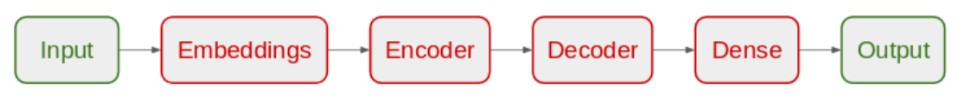
\includegraphics[width=8.5cm]{7.jpg}
    \caption{Modle Architecture}
    \label{fig:galaxy}
\end{figure}


The \textbf{encoder} takes the input sequence (in French) and encodes it into a fixed-length vector representation. This vector representation captures the meaning of the input sequence, which is then used as input to the decoder.

The \textbf{decoder} then generates the output sequence (in English) based on the encoded input representation. The decoder receives the encoded representation from the encoder and generates the output sequence one word at a time, starting with a special start-of-sentence token and ending with an end-of-sentence token.\cite{rishita2019machine}

An encoder decoder structure allows for a different input and output sequence length. First, we use an Embedding layer to create a spatial representation of the word and feed it into a LSTM layer that outputs a hidden vector, because we just focus on the output of the last time step we use return sequences is equal to False.

This output vector needs to be repeated the same number of times as the number of time step in the decoder part, for that we use the Repeat Vector layer. The decoder will be built with LSTM layer and the parameter return sequences is equal to True, so each output of the time steps is used by the Dense layer.


\begin{figure}[htp]
    \centering
    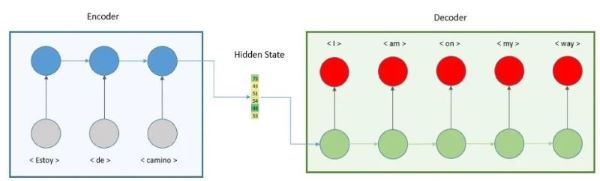
\includegraphics[width=8.5cm]{8.jpg}
    \caption{Encoder and Decoder logic using LSTM}
    \label{fig:galaxy}
\end{figure}

\textbf{Embedding} layer takes the input sequence and maps each word to a dense vector representation of units dimensions. This layer helps the model to better capture the meaning of words in the input sequence. 

\textbf{Bidirectional LSTM} layer processes the embedded input sequence in both forward and backward directions and outputs a sequence of hidden states for each time step. \cite{rathod2014machine}

\textbf{Dropout}  layer randomly drops out some of the neurons to prevent overfitting in the model. Dense layer applies a \textbf{softmax activation} function to the output of the previous layer to generate the probability distribution over the output vocabulary.

\begin{figure}[htp]
    \centering
    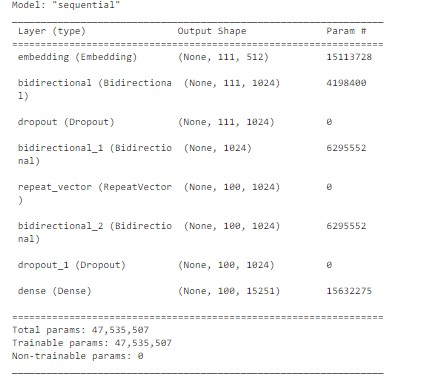
\includegraphics[width=8.5cm]{5.jpg}
    \caption{Hyper parameter tuning model}
    \label{fig:galaxy}
\end{figure}



\subsection{Evaluation}
Intrinsic evaluation focuses on intermediary objectives.\\ \textbf{BLEU (Bilingual Evaluation Understudy)} is a metric used for evaluating the quality of machine translation output against one or more reference translations. It calculates a score between 0 and 1, with higher scores indicating better translations. BLEU score is widely used in natural language processing (NLP) and machine translation evaluation. 
\cite{NIPS2014_a14ac55a}
It is used to measure the quality of text translated from a model The idea behind Bleu is to assign a single numerical score to a translation that tells us how good it is when compared to one or more human reference translations The approach that Bleu takes is to comapare the ngrams of the generated translations to the ngrams of the refrences Bleu is based on ngram precision to measure translation quality.

One can observe that the train data set When we use it the Actual and predicted both are similar.

\begin{figure}[htp]
    \centering
    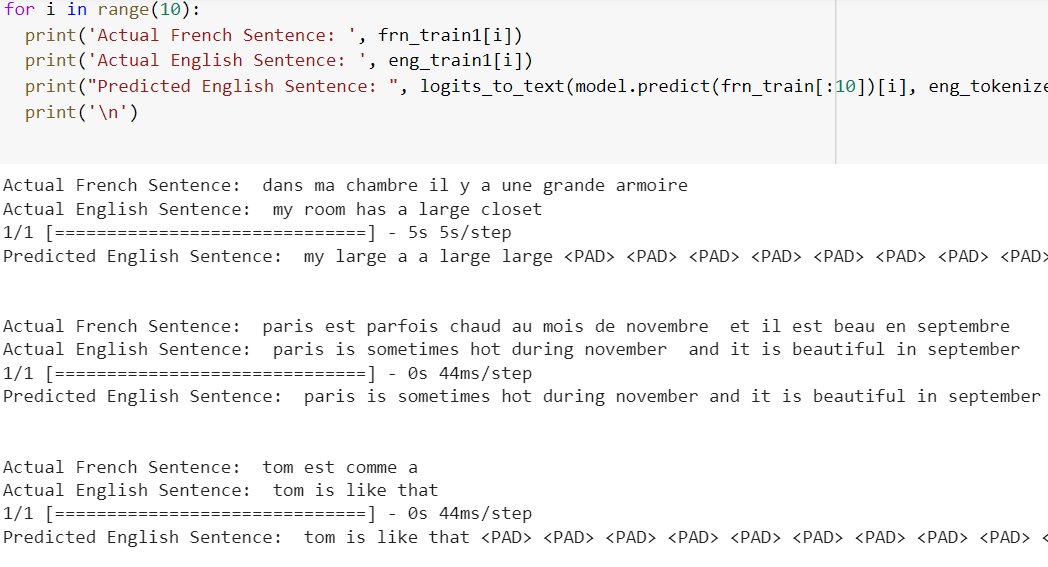
\includegraphics[width=8.5cm]{9.PNG}
    \caption{Train score predictors}
    \label{fig:galaxy}
\end{figure}

One can observe that the Test data set shows difference in actual and predicted values. For exaple actual english text is "you are luck u didn't die" but in predicted we observe "you are luck u didn't be."

\begin{figure}[htp]
    \centering
    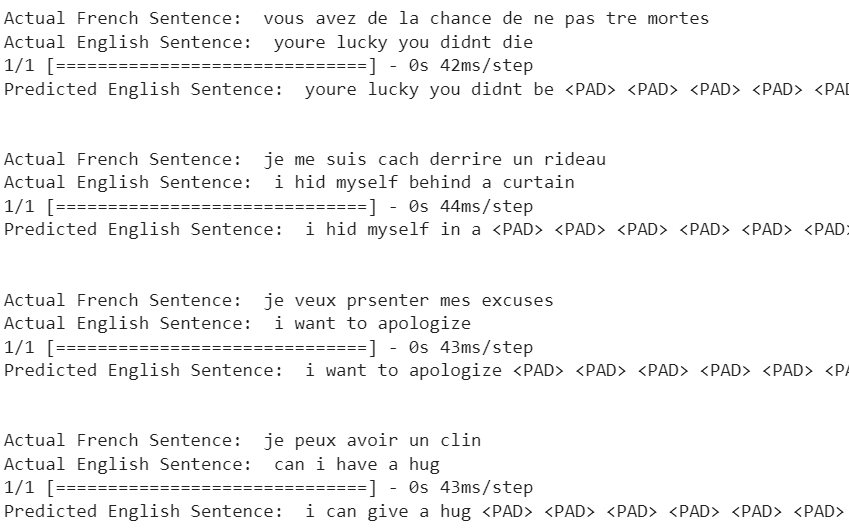
\includegraphics[width=8.5cm]{10.PNG}
    \caption{Test score predictors}
    \label{fig:galaxy}
\end{figure}


The output shows the BLEU scores for n-gram matches between the reference translation and the machine translation. The n-gram matches are computed for 1-grams (individual words), 1-2 grams (contiguous sequences of up to 2 words), 1-3 grams (contiguous sequences of up to 3 words), and 1-4 grams (contiguous sequences of up to 4 words).

In the output you provided, the BLEU scores are as follows:
\textbf{1-grams: 0.8787}
\textbf{2-grams: 0.8546}
\textbf{3-grams: 0.8450}
\textbf{4-grams: 0.8179}

These scores indicate how closely the machine translation matches the reference translation in terms of the specified n-grams. A higher score means that the machine translation contains more n-gram matches with the reference translation. 
\cite{schwenk2007smooth}
\cite{yao2018improved}
The geometric mean for n-gram in machine translation evaluation is used to combine the individual precision scores for each n-gram (1-gram, 2-gram, 3-gram, etc.) into a single score that represents the overall translation quality.

The geometric mean is computed as the nth root of the product of the individual precision scores, where n is the number of n-gram types being evaluated. For example, if we are evaluating 1-gram, 2-gram, 3-gram precision and 4-gram precision, then the geometric mean would be computed as the cube root of the product of the three individual precision scores. The formula to add is blue4 = (p1*p2*p3*p4)(1/4). The GM is 0.8487 for overall n-grams used in the model. \cite{rahit2020machine}


Regenerate response: 

\begin{figure}[htp]
    \centering
    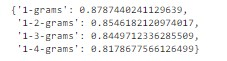
\includegraphics[width=8.5cm]{6.jpg}
    \caption{BLEU score}
    \label{fig:galaxy}
\end{figure}

\begin{figure}[htp]
    \centering
    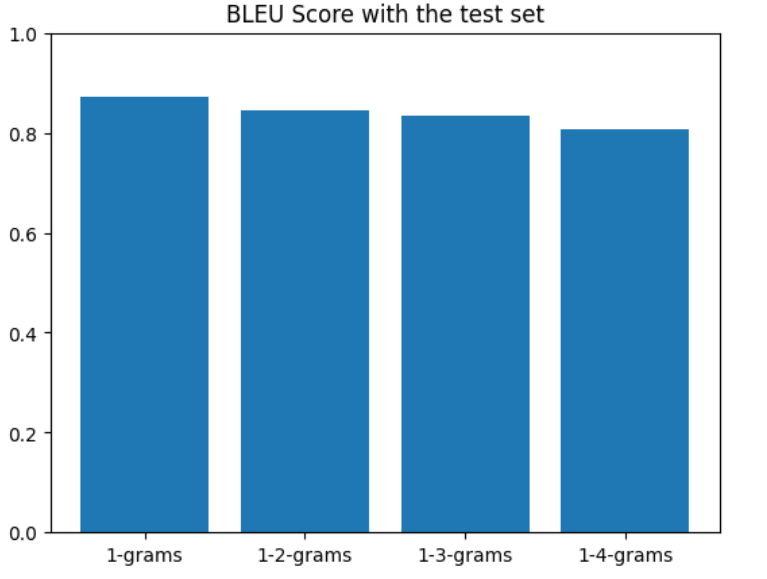
\includegraphics[width=8.5cm]{11.PNG}
    \caption{BLEU score}
    \label{fig:galaxy}
\end{figure} \\ 


\subsection{Summary and Future work}

Even though this model gives a decent result. We could improve it by increasing the number of LSTM layers in the model, instead of just three layers in the encoder and three layers in the decoder. We could also use a pre-trained embedding layer like word2vec or Glove. Finally, we could use the attention mechanism which is one of the major improvements in the natural language processing field.




% References should be produced using the bibtex program from suitable
% BiBTeX files (here: strings, refs, manuals). The IEEEbib.bst bibliography
% style file from IEEE produces unsorted bibliography list.
% -------------------------------------------------------------------------
% \bibliographystyle{IEEEbib}
% \bibliography{refs}
\bibliography{References}
\bibliographystyle{plain}

\end{document}
